\capitulo{3}{Conceptos teóricos}

En este apartado se van a explicar aquellos conceptos teóricos básicos que son necesarios para comprender el proyecto.

\section{Sistema de Información}

\subsection{Definición}

Para comenzar, hay que explicar que no existe una definición de consenso en la propia definición de Sistema de Información. De hecho, existen multitud de definiciones diferentes sobre cómo se define un Sistema de Información.

Los autores Laudon y Laudon definen un Sistema de Información como un conjunto de módulos relacionados ente sí que son capaces de obtener(o reutilizar), procesar, almacenar y distribuir cierta información para que sirva de apoyo para la toma de decisiones \cite{vicen}.
A parte de suministrar apoyo en decisiones importantes, también pueden ayudar a detectar problemas o carencias difíciles de ver sin la ayuda de estos sistemas.

\subsection{Componentes de un Sistema de Información}
Aunque existen numerosas definiciones y no existe una definición general o global, la mayoría de Sistemas de Información pueden representarse a través del diagrama de la figura \ref{fig:componentesSI}.


\imagenflotante{componentesSI}{Componentes de un Sistema de Información}

Se pueden apreciar cinco elementos principales. En primer lugar los elementos de entrada, que en nuestro proyecto serían los ficheros (.xls) originales descargados de \emph{Sigma}. 

A continuación estaría un elemento de modificación o transformación, que en nuestro caso sería el preprocesado de los ficheros originales anteriores en ficheros (.csv) reordenados, modificados y sin ningún tipo de error. También se podría incluir la carga de datos a la Base de Datos creada con anterioridad.

Seguidamente estaría el sistema de salida, donde se visualizan los resultados obtenidos. En este proyecto, el sistema de salida serían los diferentes tipos de gráficos que se pueden obtener a partir de la información que seleccione el usuario y los datos existentes o disponibles en la BBDD.

Además de estas 3 secciones, se aprecian otras dos secciones más. Una de ellas es el mecanismo de control, que es el proceso encargado de lograr los objetivos, que sería el quinto y último elemento.
En nuestro proyecto se podrían identificar numerosos mecanismos de control, como por ejemplo que los ficheros que se puedan seleccionar en los botones de \emph{Preprocesar} y \emph{Cargar Archivos} sean únicamente (.xls) y (.csv) respectivamente. Otros mecanismos de control serían la no introdución de datos repetidos en la BBDD o la selección de opciones de datos que realmente se encuentran en la BBDD, entre otros.

En cuanto a los objetivos de nuestro sistema de información, hay que destacar que se definen en el apartado anterior denominado \emph{Objetivos del proyecto}.


\subsection{Características de un Sistema de Información}

Algunas de las características más comunes que comparten casi todos los sistemas de información, son las siguientes:

\begin{itemize}
\item \textbf{Relevancia.} El sistema debe ser capaz de generar información importante y necesaria para la empresa u organización. Adicionalmente la información generada debe ser fiable\cite{estrategia}.
\item \textbf{Apoyo en la toma de decisiones.} Estos sistemas suelen ser repetitivos y capaces de soportar decisiones no estructuradas que no suelen repetirse.
\item \textbf{Flujo independiente.} Hay que destacar que en este tipo de sistemas, existe un flujo de procesamiento de datos (tanto de manera interna como externa), pero también existe un flujo independiente de los propios sistemas de información.
Estos flujos independientes suelen estar integrados a sistemas ya existentes (en el caso del proyecto, la aplicación \emph{Sigma}).
\item \textbf{Integración.} Esta característica se refiere al nexo de unión que debe existir entre el propio sistema de información y la empresa u organización. Con esta característica es más sencillo coordinar los diferentes departamentos o   divisiones, así como agilizar la toma de decisiones\cite{caracteristicas}.
\item \textbf{Control.} Esta característica no es común u obligatoria en todos los tipos de sistemas de información, pero algunos pueden contener funciones de control interno. La finalidad de este control es asegurar que la información que se genera es fiable y que los datos que se obtienen son protegidos y controlados adecuadamente.
\end{itemize}


\subsection{Tipos de Sistemas de Información}

A continuación se van a exponer los diferentes tipos de sistemas de información, desde un punto de vista empresarial.

\begin{itemize}

\item \textbf{Sistemas de procesamiento de transacciones.} Más conocido como \textbf{TPS\footnote{Transaction Processing System}} por sus siglas en inglés. Estos tipos de sistemas se categorizan como básicos, ya que son útiles a nivel operacional dentro de la organización. Es decir, se encargan de realizar transacciones diarias necesarias para el correcto funcionamiento de la empresa\cite{tipos}.
\item \textbf{Sistemas de control de procesos de negocio.} Más conocido como \textbf{BPM\footnote{Business Process Management}} por sus siglas en inglés. Estos sistemas se encargan de monitorizar y controlar procesos industriales (con la ayuda de sensores y otros dispositivos) y realizar ajustes en tiempo real que controlan los mismos.
\item \textbf{Sistemas de colaboración empresarial.} Más conocido como \textbf{ERP\footnote{Enterprise Resource Planning}} por sus siglas en inglés. Este es uno de los tipos de sistemas más utilizados, ya que prestan ayuda (como por ejemplo controlar el flujo de información) a los directivos de una empresa.
\item \textbf{Sistemas de Información Ejecutiva.} Más conocido como \textbf{EIS\footnote{Executive Information System}} por sus siglas en inglés. Estos sistemas son herramientas orientadas a usuarios de nivel gerencial, ya que generalmente permiten monitorizar estados de variables de un área determinada de la empresa a partir de información interna y externa de la misma\cite{ejecutiva}.
\item \textbf{Sistemas de Información de Gestión o Gerencial.} Más conocido como \textbf{MIS\footnote{Management Information System}} por sus siglas en inglés. Este tipo de sistemas se encargan de recopilar y procesar información de diferentes fuentes para ayudar en el proceso de toma de decisiones dentro de una empresa u organización. Estos sistemas a su vez, están orientados a solucionar problemas empresariales en general.
\end{itemize}

De los diferentes tipos de sistemas de información que se han mencionado, nuestro proyecto se asemejaría al último (\emph{Sistema de Información de Gerencial (MIS)}). Como característica curiosa, comentar que las siglas de nuestro proyecto, así como su logotipo, son las siglas de \emph{Management Information System} al revés, como se aprecia en la figura \ref{fig:logo}.

 
\subsection{Ventajas de un Sistema de Información}

Las ventajas más destacadas de un sistema de información son las siguientes:

\begin{itemize}
\item \textbf{Detección de problemas.} Gracias a un sistema de información se pueden detectar problemas para su posterior resolución.
\item \textbf{Disminución de costes.} Se disminuye el costo de mano de obra y se optimizan tiempos y tareas\cite{ventajas}. 
\item \textbf{Administración de activos.} Los activos pueden ser tangibles o intangibles. Sean del tipo que sean, los sistemas de información actuales se han convertido en una herramienta crucial para la administración de activos.
\item \textbf{Ventaja competitiva.} Los sistemas de información se han convertido en una de las principales vías para obtener ventaja competitiva en el ámbito empresarial.
\end{itemize}


\section{Gráficos Representados}

\subsection{Diagrama de Caja y Bigotes}
Los diagramas de cajas y bigotes (o diagramas de cuartiles) son un tipo de gráficas que representan una gran cantidad de información de manera muy visual y esquematizada. A su vez, se pueden apreciar características estadísticas relevantes como la simetría y la dispersión de un conjunto de datos.

Toda esta valiosa información se representa mediante unas pequeñas cajas muy intuitivas, como se aprecia en la figura \ref{fig:caja}.

%\imagenflotante{caja}{Información de Caja y Bigotes}
	
	\begin{figure}%[!h]
		\centering
		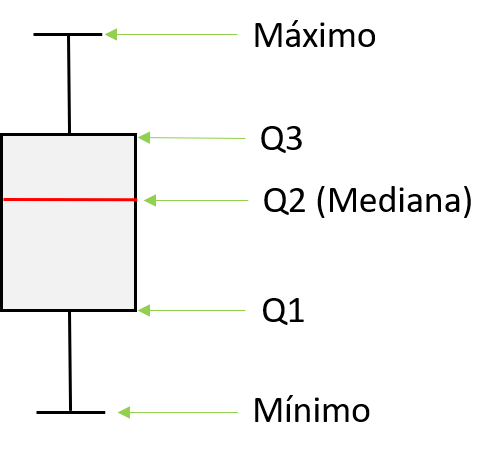
\includegraphics[width=0.6\textwidth]{caja}
		\caption{Información de Caja y Bigotes}\label{fig:caja}
	\end{figure}
	
Se diferencian cinco partes fundamentales: 
\begin{itemize}
	\item 
	\textbf{Tres Cuartiles (Q1, Q2 y Q3).} Hay que destacar que el segundo cuartil(Q2) coincide con la mediana y representa la relación entre el primer y tercer cuartil. El primer cuartil identifica el valor por debajo del cual queda un 25\% de todos los datos de la muestra ordenada. Del mismo modo, el tercer cuartil es el valor por debajo del cual quedan el 75\% de los datos de la muestra.
	\item 
	\textbf{Máximo.} Representa el valor máximo de los datos.
	\item 
	\textbf{Mínimo.} Representa el valor mínimo de los datos.
\end{itemize}

A continuación, en la figura \ref{fig:grafico2} se puede apreciar un diagrama de caja y bigotes que se genera mediante nuestra aplicación, donde se pueden observar los conceptos teóricos anteriormente mencionados. 

\begin{figure}%[!h]
		\centering
		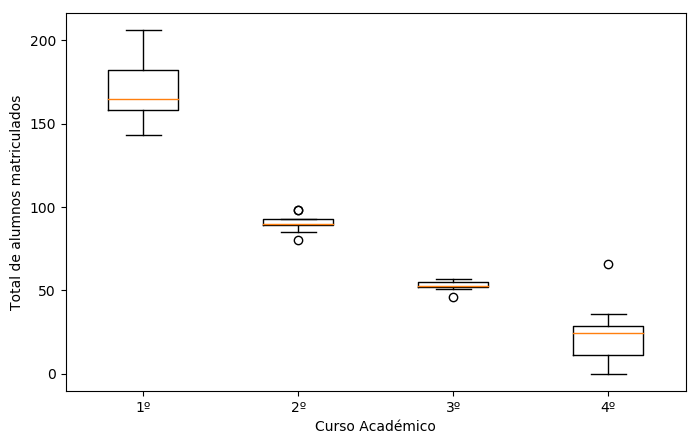
\includegraphics[width=0.9\textwidth]{grafico2}
		\caption{Diagrama de Caja y Bigotes}\label{fig:grafico2}
	\end{figure}


\subsection{Gráfico de Barras}

Los  gráficos de barras son un tipo de representación gráfica realizada en un eje cartesiano de las frecuencias de una variable cualitativa o discreta. \cite{ine}

En uno de los ejes se posicionan las diferentes categorías de la variable cualitativa (en el caso de nuestro proyecto, las asignaturas de un determinado curso) y en el otro eje se posiciona la frecuencia de cada asignatura (en nuestro proyecto sería la cantidad de alumnos matriculados).

La orientación del gráfico puede ser horizontal o vertical. Hay que destacar que en nuestro proyecto se utiliza un \textbf{gráfico apilado y horizontal}. Es decir, las diferentes asignaturas del curso seleccionado se sitúan en el eje vertical y las barras apiladas de los diferentes grupos (teóricos o prácticos) aumentan horizontalmente.

Este tipo de distribución horizontal se suele utilizar cuando existen numerosas categorías o el nombre de las mismas es demasiado extenso, como es el caso (generalmente hay diez asignaturas por curso).

Hay que destacar que en los gráficos apilados, las diferentes barras se dividen en segmentos de diversos colores (para poder apreciarlos y diferenciarlos del resto) y cada uno de estos colores, representa una serie. En nuestro caso, estas series se corresponden con los diferentes grupos (teóricos o prácticos) que componen las asignaturas. A continuación, en la figura \ref{fig:grafico1T} se pueden apreciar todos los conceptos en un gráfico obtenido por nuestra aplicación. 

\begin{figure}%[!h]
		\centering
		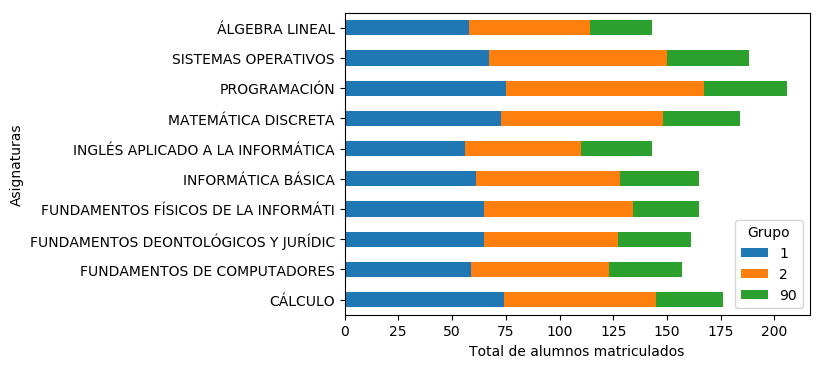
\includegraphics[width=0.9\textwidth]{grafico1T}
		\caption{Gráfico apilado horizontalmente de asignaturas por curso}\label{fig:grafico1T}
	\end{figure}